\documentclass[10pt]{article}
\usepackage{amsthm}
\usepackage{graphicx}
\usepackage{subfig}
\usepackage{physics}

\graphicspath{ {figures/} }
\begin{document}

The Monte Carlo simulation models a layered AFM insulator with four antiferromagnetically coupled layers, each composed of $N \times N$ spins. A single-spin Metropolis algorithm is used and energy
fluctuations are determined by the system Hamiltonian,
$$H = -J_{FM}\sum_{l}\sum_{<i,j>}\vec{S}_{l,i}\cdot \vec{S}_{l,j} + J_{AFM}\sum_{l < N}\sum_{i}\vec{S}_{l,i} \cdot \vec{S}_{l+1,i} + K\sum_{l,i}\left (S_{l,i,z}\right )^{2} - B \sum_{l,i}S_{l,i,z}$$
where $\vec{S}_{l,i}$ is the spin unit vector residing on site $i$ of layer $l$. The $J_{FM}$ term characterizes intra-layer
ferromagnetic interactions and the $J_{AFM}$ term characterizes antiferromagnetic coupling between layers. The $K$ term describes
easy-axis anisotropy (for $K < 0$) and the $B$ term describes Zeeman coupling.
In our simulations, $J_{FM} = 1$ and magnetization per spin is calculated by averaging the $S_{i,z}$ components of each spin on either an individual layer or over the whole system.
When sweeping the external field strength, magnetization per spin is measured over the entire system as well as on each individual layer. Mean magnetization per spin measurements
are calculated by averaging the mean $S_{i,z}$ value over 1000 ensembles at the indicated external field strength.

As mentioned in the main text, applying a gate voltage to the top and/or bottom of the system breaks inversion symmetry. This effect is modeled in our simulation by adjusting the anisotropy $K$ and/or interlayer
coupling strengths $J_{AFM}$ on the top and bottom layers [Note: need to further investigate effect of symmetry breaking via $J_{FM}$ ]. When sweeping the magnetic field strength in a system that exhibits
inversion symmetry (i.e. uniform parameters throughout every layer), we observe any of the patterns of Figure 1 with equal probability.

\begin{figure}[!htb]
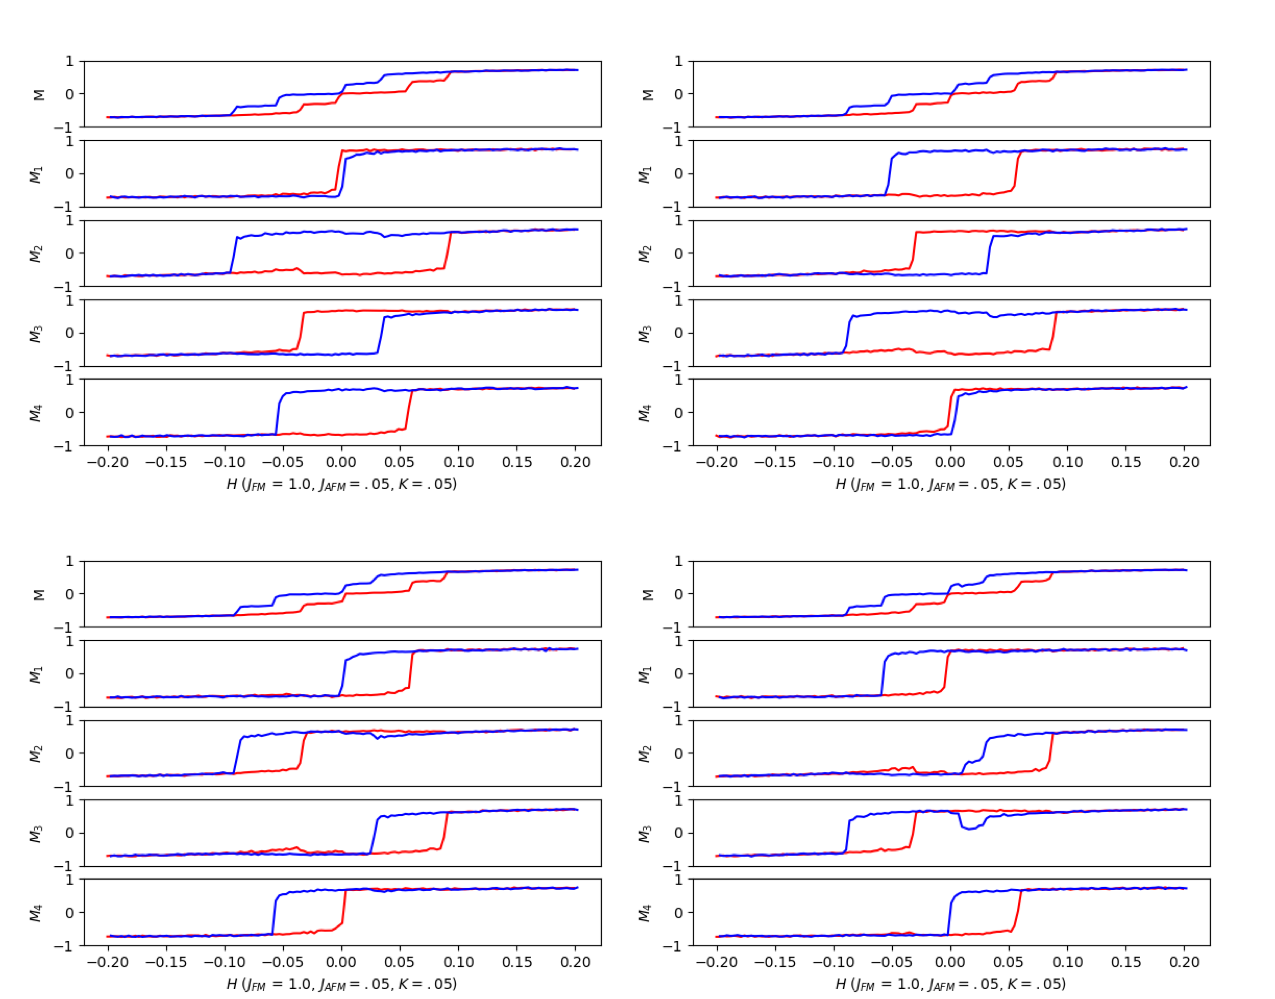
\includegraphics[width=\textwidth]{4_patterns.png}
\caption{The four possible switching patterns obtained for a symmetric system when sweeping the magnetic field. The red line indicates sweeping in the positive direction, and the blue line indicates
sweeping in the negative direction. [Note: Will replace with improved figures - just a representation for now]. }
\end{figure}

One representative approach for breaking inversion symmetry is to increase the anisotropy $K$ on the top layer only, as seen in Figure 2. In doing so, we observe behavior similar to that seen in Figure 2b in the main text. That is,
when reversing the sweeping direction, the preferred bistable state in the intermediate magnetic field region is switched. We can obtain similar behavior by increasing $J_{AFM}$ between the top two layers, as seen in Figure 3.

\begin{figure}[!htb]
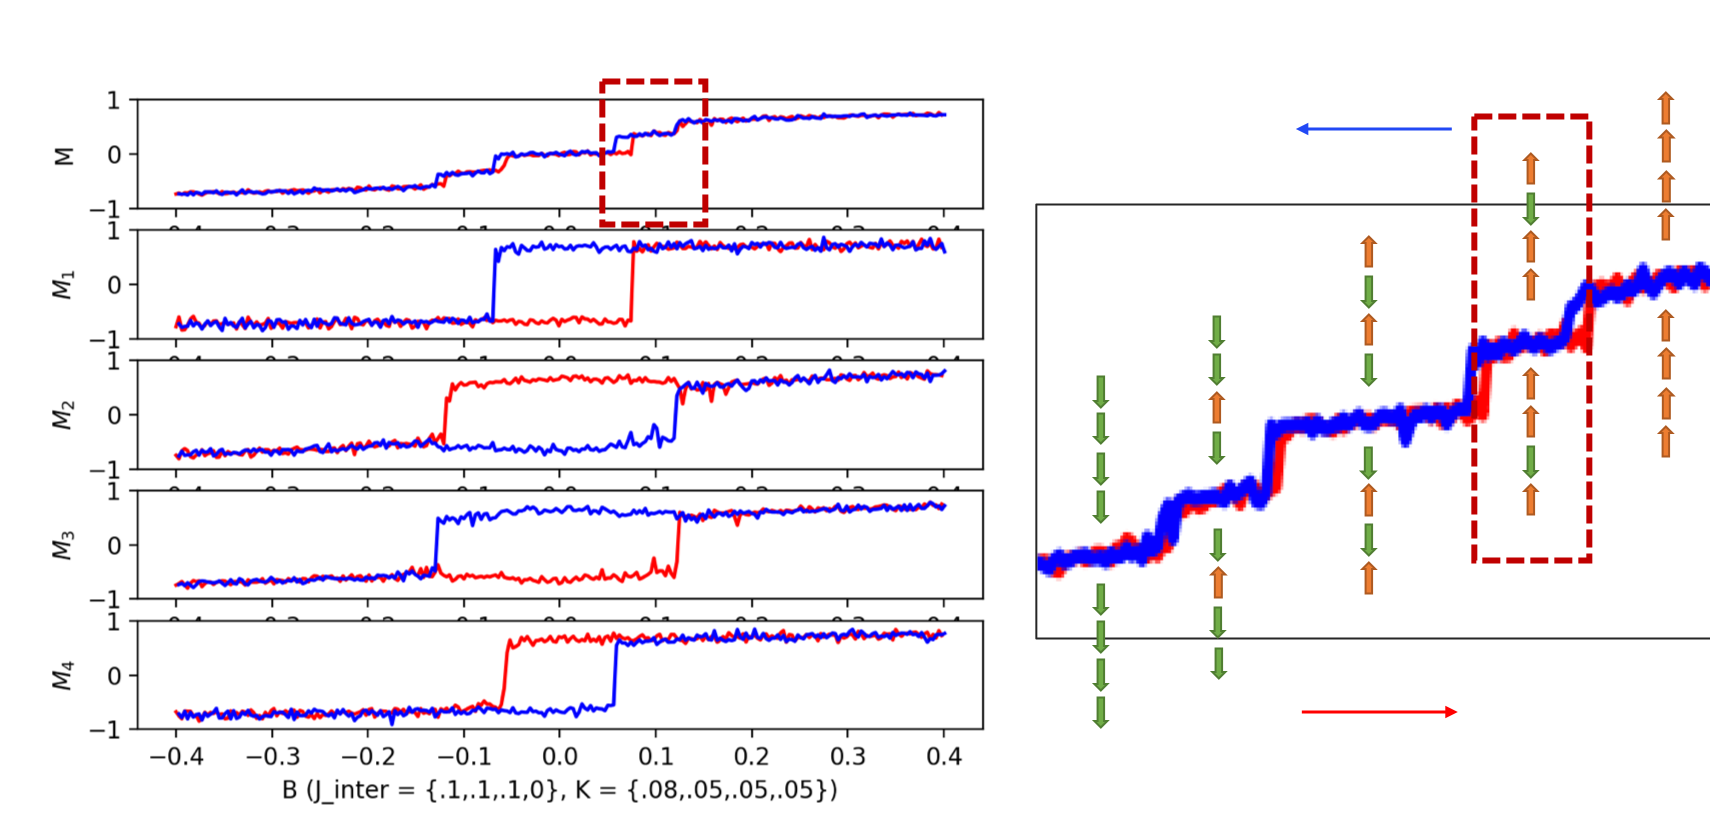
\includegraphics[width=\textwidth]{bistable.png}
\caption{In this simulation, the anisotropy of the top layer is increased slightly to $K_{1} = .08$ while the other layers have an anisotropy of $K = .05$. The values of
$J_{FM}$ and $J_{AFM}$ are uniform throughout the system. The dashed lines highlight the bistable state switching observed: during the positive sweep,  $\uparrow \uparrow \downarrow \uparrow$
is preferred while  $\uparrow \downarrow \uparrow  \uparrow$ is preferred during the negative sweep [Note: Will replace with improved figures - just a representation for now]. }
\end{figure}

\begin{figure}[!htb]
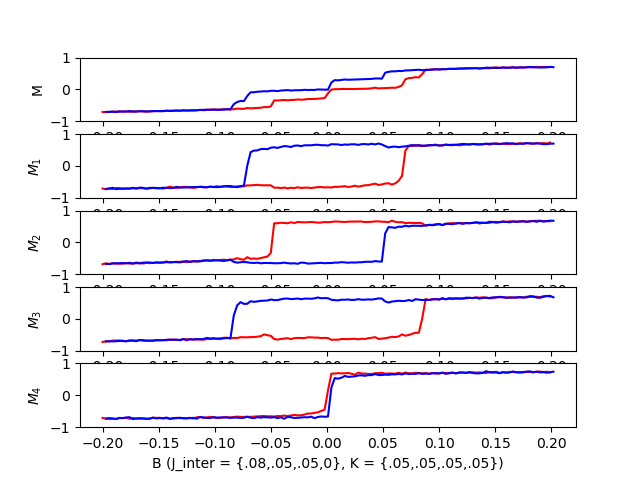
\includegraphics[width=\textwidth]{sim_6.png}
\caption{In this simulation, the interlayer coupling strength of the top two layers is increased slightly to $J_{AFM,12} = .08$ while the other layers have a coupling strength of $J_{AFM} = .05$. The values of
$J_{FM}$ and $K$ are uniform throughout the system. [Note: Will replace with improved figures - just a representation for now]. }
\end{figure}


[Note: this section is not yet confirmed. These are just my current thoughts. Will update as needed when simulation results are ready] When there is considerable imbalance in the system
parameters, we begin to see a transition from the behavior described in Figure 2b of the main text to that of Figure 2a or 2c. That is, the preferred bistable state in the intermediate magnetic field region
will no longer depend on the sweeping direction. As an example, if we increase $J_{AFM}$ to $.3$ between the top two layers (as opposed to $J_{AFM} = .08$ in Figure 3), the results of sweeping the magnetic field
are similar to those obtained in Figure 2c of the main text. Specifically, we observe that $\uparrow \downarrow \uparrow  \uparrow$ is preferred in the positive intermediate field region during both the positive
and negative sweep of the magnetic field.

\begin{figure}[!htb]
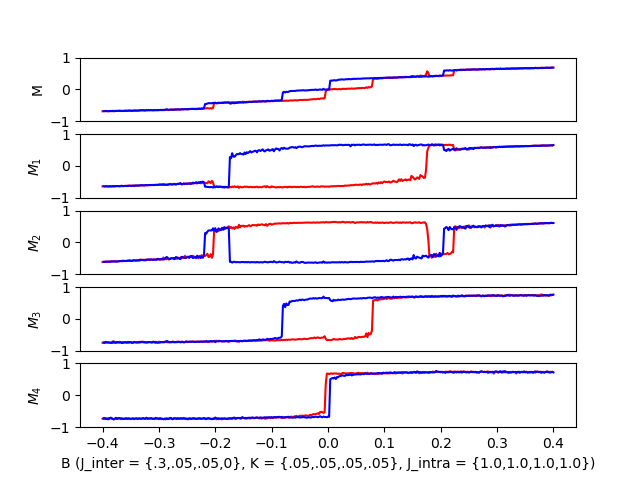
\includegraphics[width=\textwidth]{sim_92.png}
\caption{In this simulation, the interlayer coupling strength of the top two layers is increased slightly to $J_{AFM,12} = .08$ while the other layers have a coupling strength of $J_{AFM} = .05$. The values of
$J_{FM}$ and $K$ are uniform throughout the system. [Note: Will replace with improved figures - just a representation for now]. }
\end{figure}

\end{document}



%%As mentione din the main text, top and bottom gate break inversion symmetry, which in our simulation can be simulated by adjusting the anisotropy and interlayer coupling strength. Breaking intralayer symmetry
%%By changing either inter or anisotropy we can reproduce the pattern seen in B. To realize 2a or c, we can to combine the symmetry breaking effects. Finally we tried changing intra layer to see.
